
\documentclass[12pt,a4paper]{article} 

\usepackage{float,times,graphicx,mathtools}
\usepackage{amsmath}
\usepackage{amsfonts}
\usepackage{amssymb}
\usepackage{latexsym}
\usepackage{epsfig}
\usepackage{graphicx}
\usepackage{caption}
\usepackage{subcaption}
\usepackage{color}
\usepackage{pdfpages}
\usepackage{natbib}
\usepackage[space]{grffile}
\usepackage{wrapfig}
\usepackage{subcaption}
\usepackage{url}
\usepackage{bbm}

\DeclareMathOperator{\logit}{logit}
\DeclareMathOperator{\tr}{tr}
\bibpunct[, ]{(}{)}{;}{a}{,}{,}
\graphicspath{{../}}  
\addtolength{\oddsidemargin}{-1in}
	\addtolength{\evensidemargin}{-1in}
	\addtolength{\textwidth}{1.75in}
	\addtolength{\topmargin}{-1.3in}
	\addtolength{\textheight}{2in}
\date{\vspace{-5ex}}
\begin{document}

\begin{itemize}

\end{itemize}
\begin{itemize}
\item the estimated $_{45}q_{15}$ are now more stable and flat in the pre-DHS periods, after imposing AR(1) priors on the parameters of the LogQuad model (instead of RW on last Friday) as well as AR(1):AR(1) priors on $g_x$
\item estimated $_{45}q_{15}$ lower than WPP estimates in the pre-DHS periods
\item check estimated $g_x$ and $mortality schedules$
\item compared to the RW model, the AR on $m_x$ with AR(1):AR(1) on $g_x$ estimated much less variations in the mortality schedules over time. In particular, estimated improvements were higher under the RW model (of course for males that seems to be exaggerated given the estimated $_{45}q_{15} \sim 0.8$ in 1960 previously)
\item estimated migration proportions at the highest age groups still seem to be unreasonable, especially in the earliest years
	\begin{itemize}
  \item[--] allow prior on population counts to increase at the oldest ages / use probabilistic ccmpp instead of deterministic such that at the oldest ages the projected counts are with higher uncertainty
	\item[--] allow more diffused priors on the mortality rates at the oldest ages (need to simulate and check what the uncertainty of the LogQuad model is at different age ranges)
	\item[--] stricter prior on $g_x$ at the infant and the oldest ages
	\end{itemize}
\item currently using the same prior mean of the migration proportions from the package, where at the middle age groups (15-54) they are -0.055 and 0 elsewhere, i.e. the AR(1):AR(1) process are centered around different means, instead of being penalising towards the same level
\item ARIMA(1,1,0) or AR(1) around a linear trend for h (and k?)
\end{itemize}

\paragraph{\textcolor{red}{My} intuition on separable AR(1):AR(1) processes} \\~\\

Separability is defined through the kronecker product of the precision matrices of the two dimensions. For example, given random variables $Y_{x,t}$ over a 2-D space, say age ($x$) and time ($t$), assuming the correlation along the age and time dimensions each follow an AR(1) process with $\rho_x$ and $\rho_t$, then the correlation between $Y_{x_1, t_1}$ and $Y_{x_2, t_2}$ under the separably constructed precision precision (covariance) matrix is $\rho_x^{dx} \rho_t^{dt}$ (\textit{The comprehensive TMB documentation}). 

Let $\boldsymbol{Y}$ be the matrix of random variables $Y_{x,t}$ where rows correspond to different ages and columns correspond to different years, define $\boldsymbol{y}$ as the vectorised $\boldsymbol{Y}$ in column major order, i.e. 
\begin{align*}
\boldsymbol{y} = \begin{pmatrix} \boldsymbol{y}_{x1} \\ \boldsymbol{y}_{x2} \\ \vdots \\ \boldsymbol{y}_{xT} \end{pmatrix},
\end{align*}
 then the precision matrix of $\boldsymbol{y}$ is expressed as $\boldsymbol{V} = \boldsymbol{V}_t(\rho_t) \otimes \boldsymbol{V}_x(\rho_x)$ (note that order is reversed!), where $\boldsymbol{V}_x(\rho_x)$ and $\boldsymbol{V}_t(\rho_t)$ are the precision matrices of the AR(1) processes along the age and time dimensions respectively, dependent on parameters $\rho_x$ and $\rho_t$.

Define $\boldsymbol{D}_x(\rho_x)$ to be the square root of $\boldsymbol{V}_x(\rho_x)$ such that $\boldsymbol{V}_x = \boldsymbol{D}_x'\boldsymbol{D}_x$ (similarly for the time dimension), then $\boldsymbol{V} = \boldsymbol{V}_t \otimes \boldsymbol{V}_x = (\boldsymbol{D}_t'\boldsymbol{D}_t) \otimes (\boldsymbol{D}_x'\boldsymbol{D}_x) = (\boldsymbol{D}_t' \otimes \boldsymbol{D}_x')(\boldsymbol{D}_t \otimes \boldsymbol{D}_x) = (\boldsymbol{D}_t \otimes \boldsymbol{D}_x)' (\boldsymbol{D}_t \otimes \boldsymbol{D}_x)$.

Under AR(1), we have (also for the time dimension)
\begin{align*}
\boldsymbol{D}_x = \begin{pmatrix} -\rho_x & 1 & 0 & 0 & \dots \\
																		  0 & -\rho_x & 1 & 0 & \\
																			0 & 0 & -\rho_x & 1 \\
																		  \vdots & & \ddots  & &  \\
																			\end{pmatrix}
\end{align*}
and
\begin{align*}
\boldsymbol{D}_t \otimes \boldsymbol{D}_x = \begin{pmatrix} \rho_t \rho_x & -\rho_t & 0 & 0 & \dots & -\rho_x & 1 & 0 & 0 &\dots \\
 0 & \rho_t \rho_x & -\rho_t & 0 & \dots & 0 & -\rho_x & 1 & 0 & \dots \\
\vdots & & & \ddots \end{pmatrix}.
\end{align*}

Therefore, penalty imposed by the separably constructed AR(1):AR(1) is \textbf{proportional to}
\begin{align*}
\boldsymbol{y}'\boldsymbol{V}\boldsymbol{y} \, &= \boldsymbol{y}' (\boldsymbol{V}_t \otimes \boldsymbol{V}_x) \boldsymbol{y} \\
&= \boldsymbol{y}' (\boldsymbol{D}_t \otimes \boldsymbol{D}_x)' (\boldsymbol{D}_t \otimes \boldsymbol{D}_x) \boldsymbol{y} \\
&= \sum \limits_{j=1}^{T-1} \sum \limits_{i=1}^{X-1} (y_{i+1, j+1} - \rho_x \, y_{i, j+1} - \rho_t \, y_{i+1,j} + \rho_t \rho_x \, y_{i, j})^2
\end{align*}

Intuitively, $y_{x+1, t+1} \, \vert \, y_{x,t}, y_{x+1,t}, y_{x,t+1}$ is penalised towards $\rho_x \, y_{i, j+1} + \rho_t \, y_{i+1,j} - \rho_t \rho_x \, y_{i, j}$. Alternatively, this is equivalent to penalising $y_{x+1, t+1} - \rho_x \, y_{x, t+1}$ towards $\rho_t \, (y_{x+1, t} - \rho_x \, y_{x, t})$.
\\~\\
It might be easier to first consider the limiting case when $\rho_x = 1$ and $\rho_t = 1$, i.e. a RW(1):RW(1) (also similar to a cross age-time first order penalty in 2D tensor P-spline). Then then separable precision matrix is penalising $\underbrace{y_{x+1, t+1} - y_{x, t+1}}_\substack{\text{increment from age $x$} \\ \text{ to $x+1$ in year $t+1$}}$ towards $\underbrace{y_{x+1, t} - y_{x, t}}_\substack{\text{increment from age $x$} \\ \text{to $x+1$ in year $t$}}$. 
\\~\\
In other words, changes in levels of $y_{x,t}$ across neighbouring ages should be similar across neighbouring years. The transition onto an AR(1):AR(1) means that the dependencies across ages and years are weaker, and in our case (AR(1):AR(1) on migration proportions $g_{x,t}$) being drawn to 0 (or the corresponding mean at each age-time location). Specifically, in each year, $y_{x+1, t}$ should be close to $\rho_x \, y_{x,t}$, and the deviations in the age direction should be close to $\rho_t$ times the deviations in the previous year at the corresponding ages.

\\~\\
Additional one dimensional AR(1) precisions/penalties need to be added to the boundaries, i.e. 
\begin{itemize}
\item[1)] AR(1) in the age direction in the first year on $\boldsymbol{y}_{x,1}$,
\item[2)] AR(1) in the time direction in the first age on $\boldsymbol{y}_{1,t}$,  as well as 
\item[3)] a prior on $y_{1,1}$ to complete the rank.
\end{itemize}

For any one dimensional AR(1) processes, what TMB does when using \textit{AR1\_t} is that it assumes initial state $y_1 = \varepsilon_1 \sim N(0, \frac{\sigma^2}{1-\rho^2})$, i.e. variance of the initial state follows the marginal variance of an stationary AR(1) process. In particular, normally we have
\begin{align*}
y_1 &= \varepsilon_1 \sim N(0, \frac{\sigma^2}{1-\rho^2}) \\
y_2 &= \rho \, y_1 + \varepsilon_2, \quad \varepsilon_2 \sim N(0, \sigma^2) \\
&\vdots
\end{align*}

Under TMB's formulation, it is
\begin{align*}
y_1 &= \varepsilon_1^* \sim N(0, \frac{\sigma^2}{1-\rho^2}) \\
y_2 &= \rho \, y_1 + \sqrt{1-\rho^2} \, \varepsilon_2^*, \quad \varepsilon_2^* \sim N(0, \frac{\sigma^2}{1-\rho^2}) \\
&\vdots
\end{align*}
so that the marginal variances of the $\boldsymbol{y}$ can be inputted directly. This means that the precision matrix using \textit{AR1\_t} is essentially $\boldsymbol{D}^* ' \boldsymbol{D}^*$, where

\begin{align*}
\boldsymbol{D}^* = \underbrace{\begin{pmatrix} 1 & 0 & 0 & 0 & \dots \\
																	0 & \frac{1}{\sqrt{1-\rho^2}} & 0 & 0 & \dots \\
																	0 & 0 &\frac{1}{\sqrt{1-\rho^2}} & 0 \\
																	\vdots & & \ddots \end{pmatrix}}_{\substack{\text{square roots of inverse weights} \\ \text{ of the variances of \boldsymbol{\varepsilon}}}} \underbrace{\begin{pmatrix} \color{red}1 & \color{red} 0 & \color{red}0 & \color{red}0 & \color{red}\dots \\
																	-\rho & 1 & 0 & 0 & \dots \\
																	0 & -\rho & 1 & 0 & \\
																	0 & 0 & -\rho & 1 & \\
																	\vdots & & \ddots \end{pmatrix}}_{\text{inverse transformation from \boldsymbol{y} to \boldsymbol{\varepsilon}}}
\end{align*}
$\implies$ when $\boldsymbol{y}$ is passed to compute the density, it is first transformed to the $\boldsymbol{\varepsilon^*}$ scale which are i.i.d Normal, and then weights them according to the variances. Note the added first row that gives prior to the boundary and hence the rank is full.

Therefore when using \textit{SEPARABLE( AR1, AR1)} the Kronecker product is full. However compared to just above with the added priors on boundary, \textit{SEPARABLE( AR1, AR1)} has additional one-dimensional AR(1) penalties on $\sum_t \sum_i (y_{i+1,t} - \rho_x y_{i,t})^2$ and $\sum_t \sum_i (y_{i,t+1} - \rho_t y_{i,t})^2$.

\\~\\
\textit{SCALE( SEPARABLE( AR1, AR1 ), $\sigma$)} or \\
\textit{SEPARABLE( SCALE( AR1, $\sigma_t$ ), SCALE( AR1, $\sigma_x$))} or \\
\textcolor{red}{(probably redundant as the $\rho_x$'s and $\rho_t$'s already serve as weights between the age and time dimensions)} \\
\textit{SCALE( SEPARABLE( SCALE( AR1, $\sigma_t$ ), SCALE( AR1, $\sigma_x$)), \sigma)} 


\newpage
\centering \paragraph{Results} \\~\\
\begin{figure}[H]
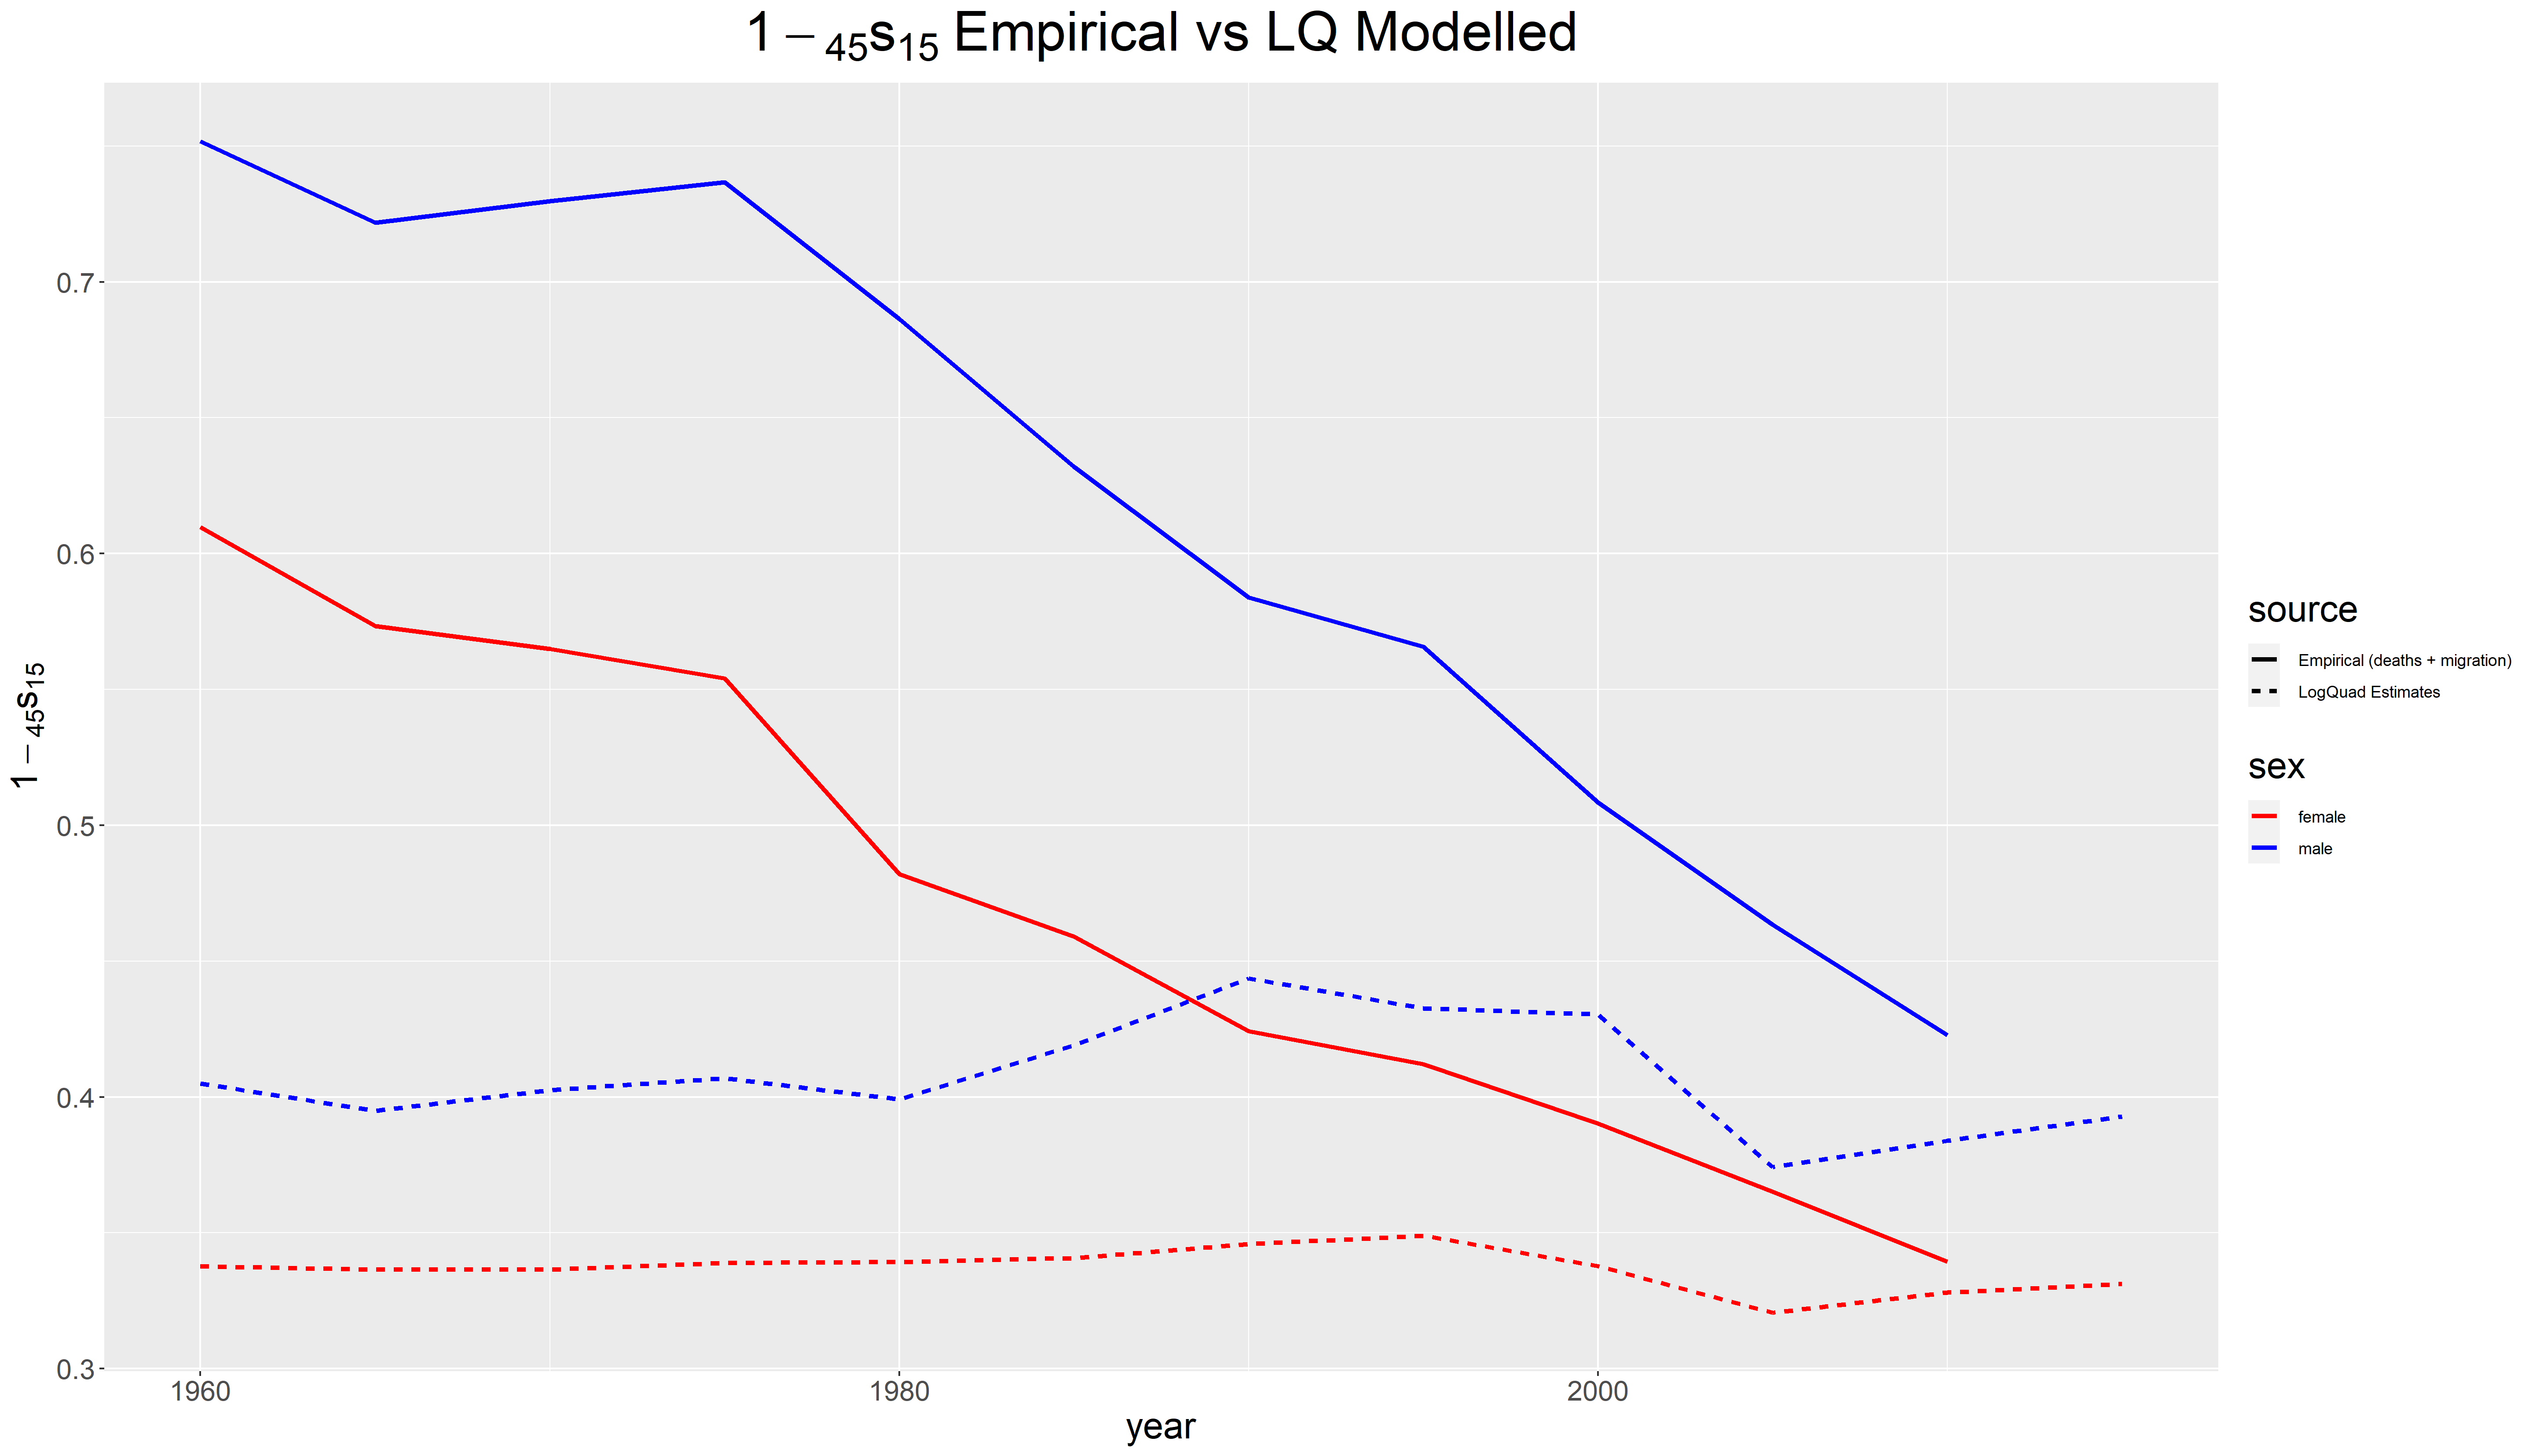
\includegraphics[width=\linewidth]{Burkina Faso/2/CCMPP 1-s4515.png}
\end{figure}
\begin{figure}[H]
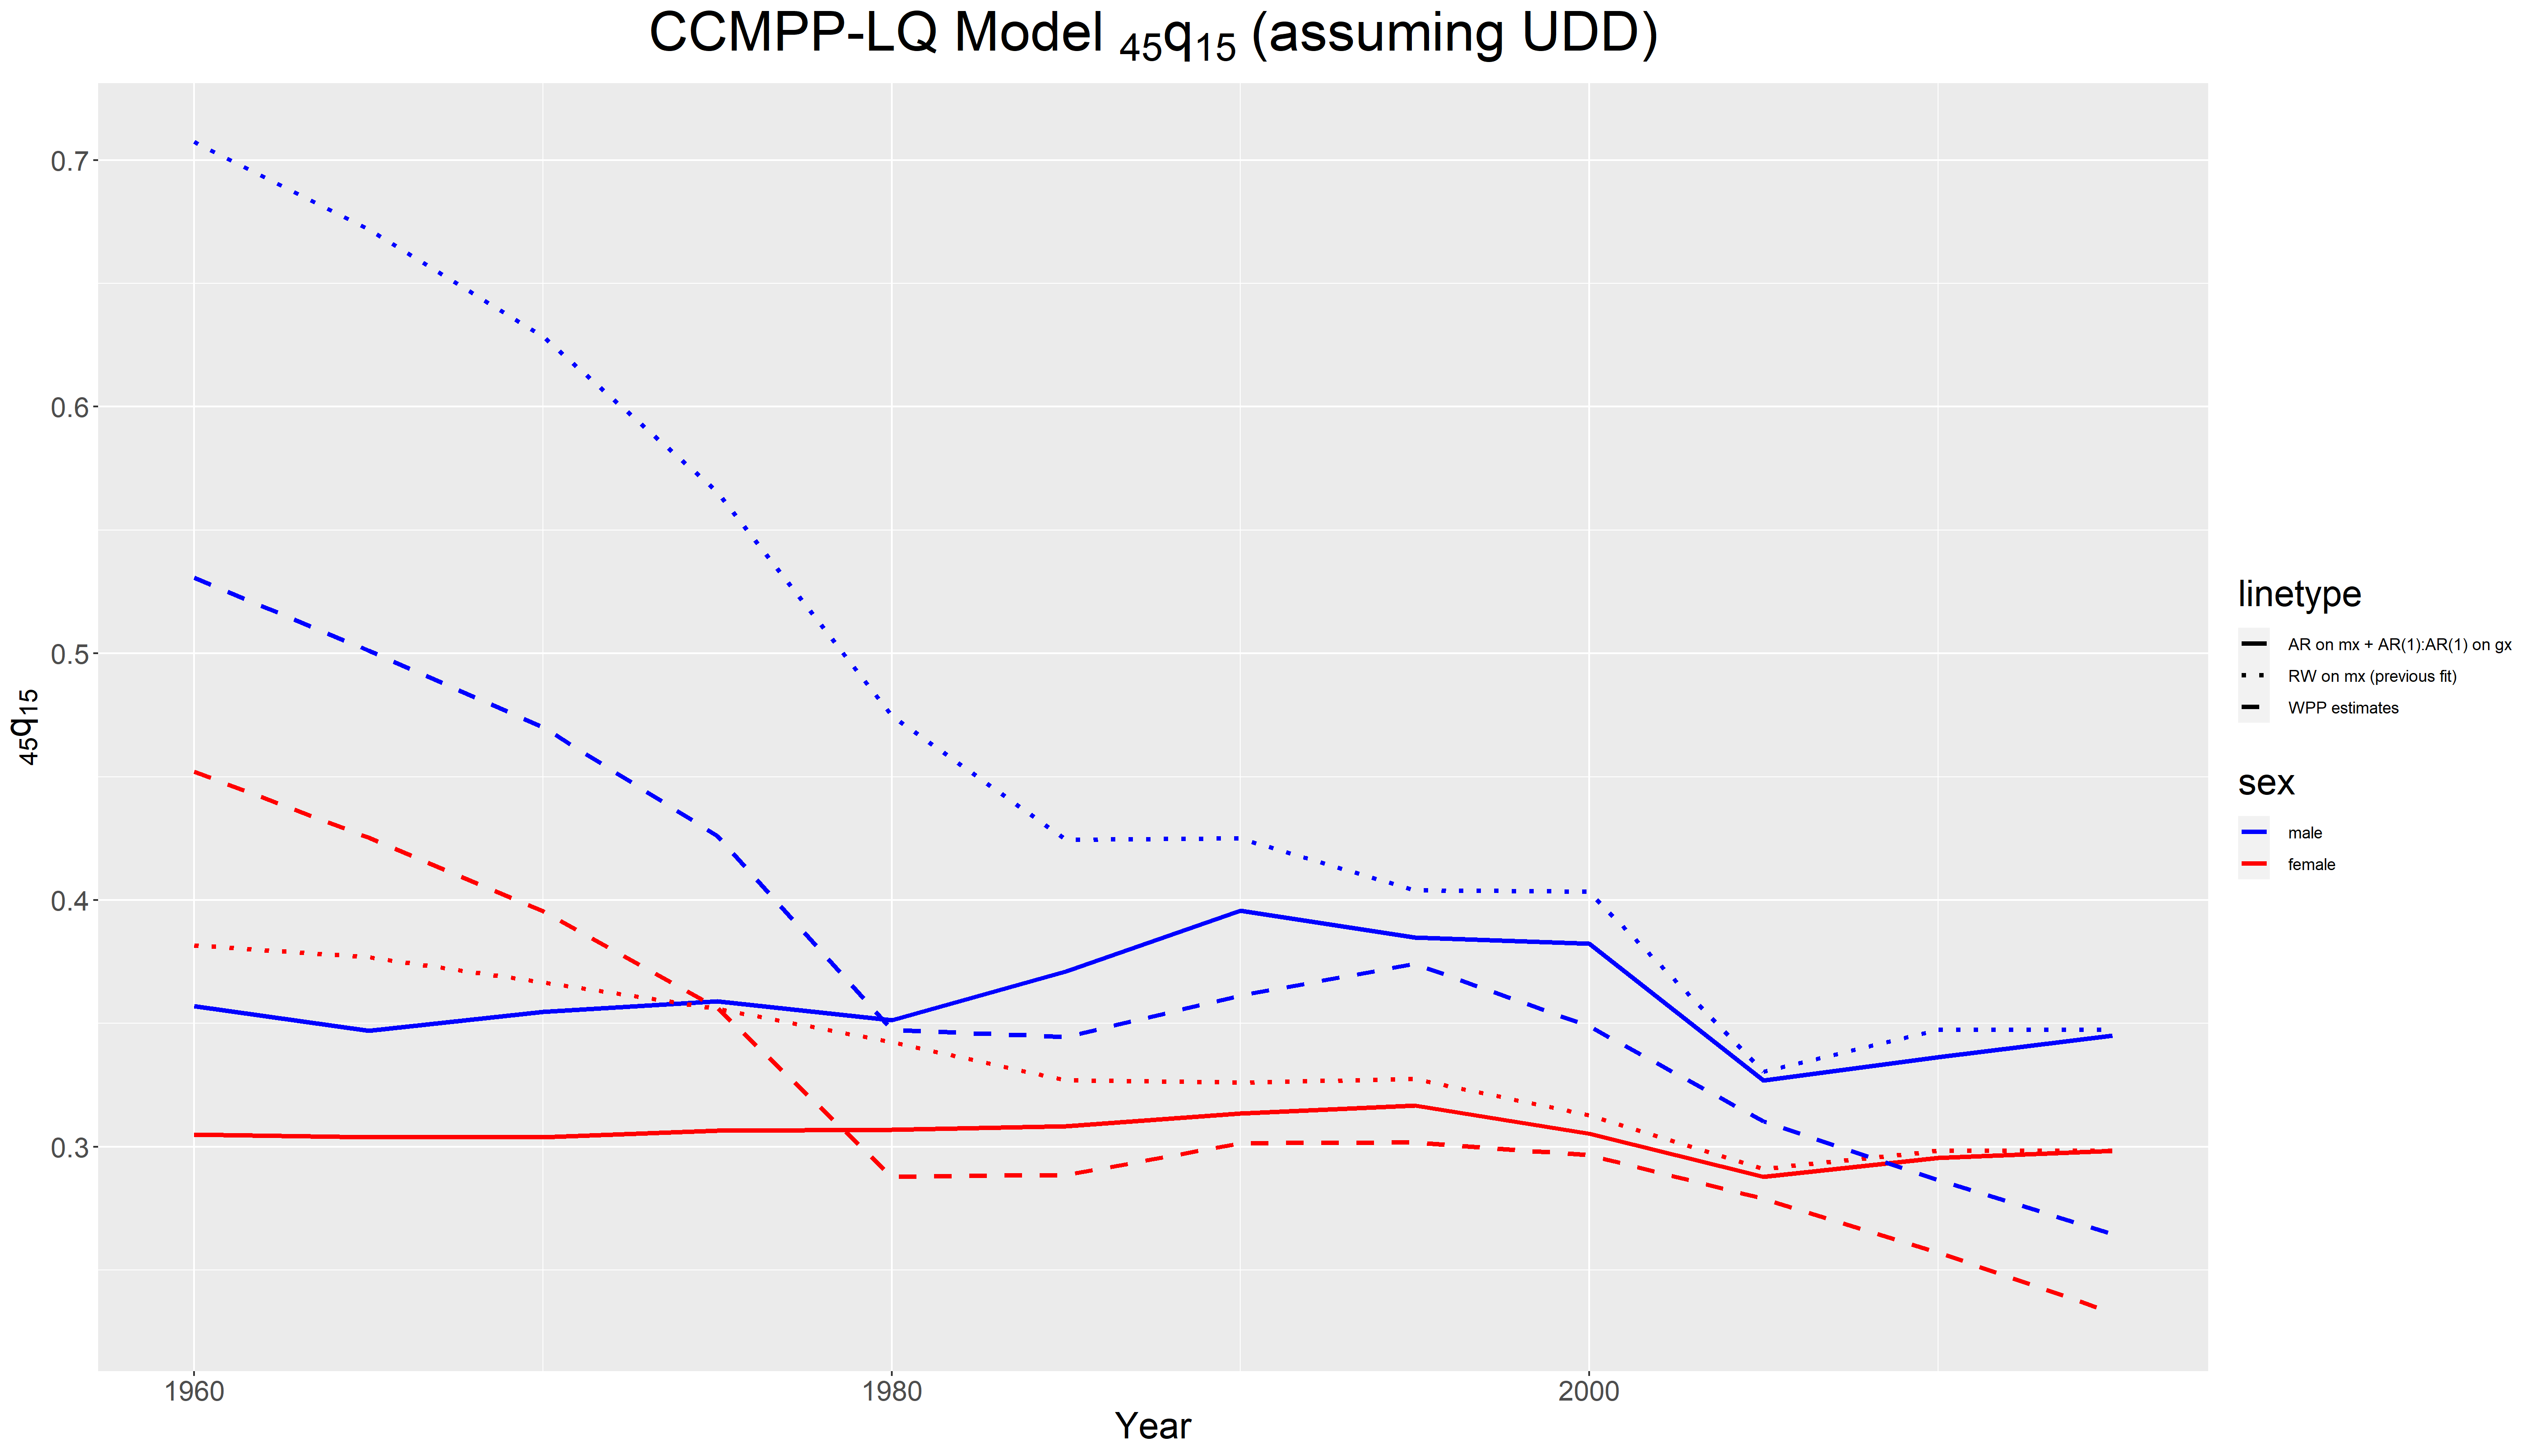
\includegraphics[width=\linewidth]{Burkina Faso/2/CCMPP q4515 compare WPP and RW.png}
\end{figure}

\newpage
\begin{figure}[H]
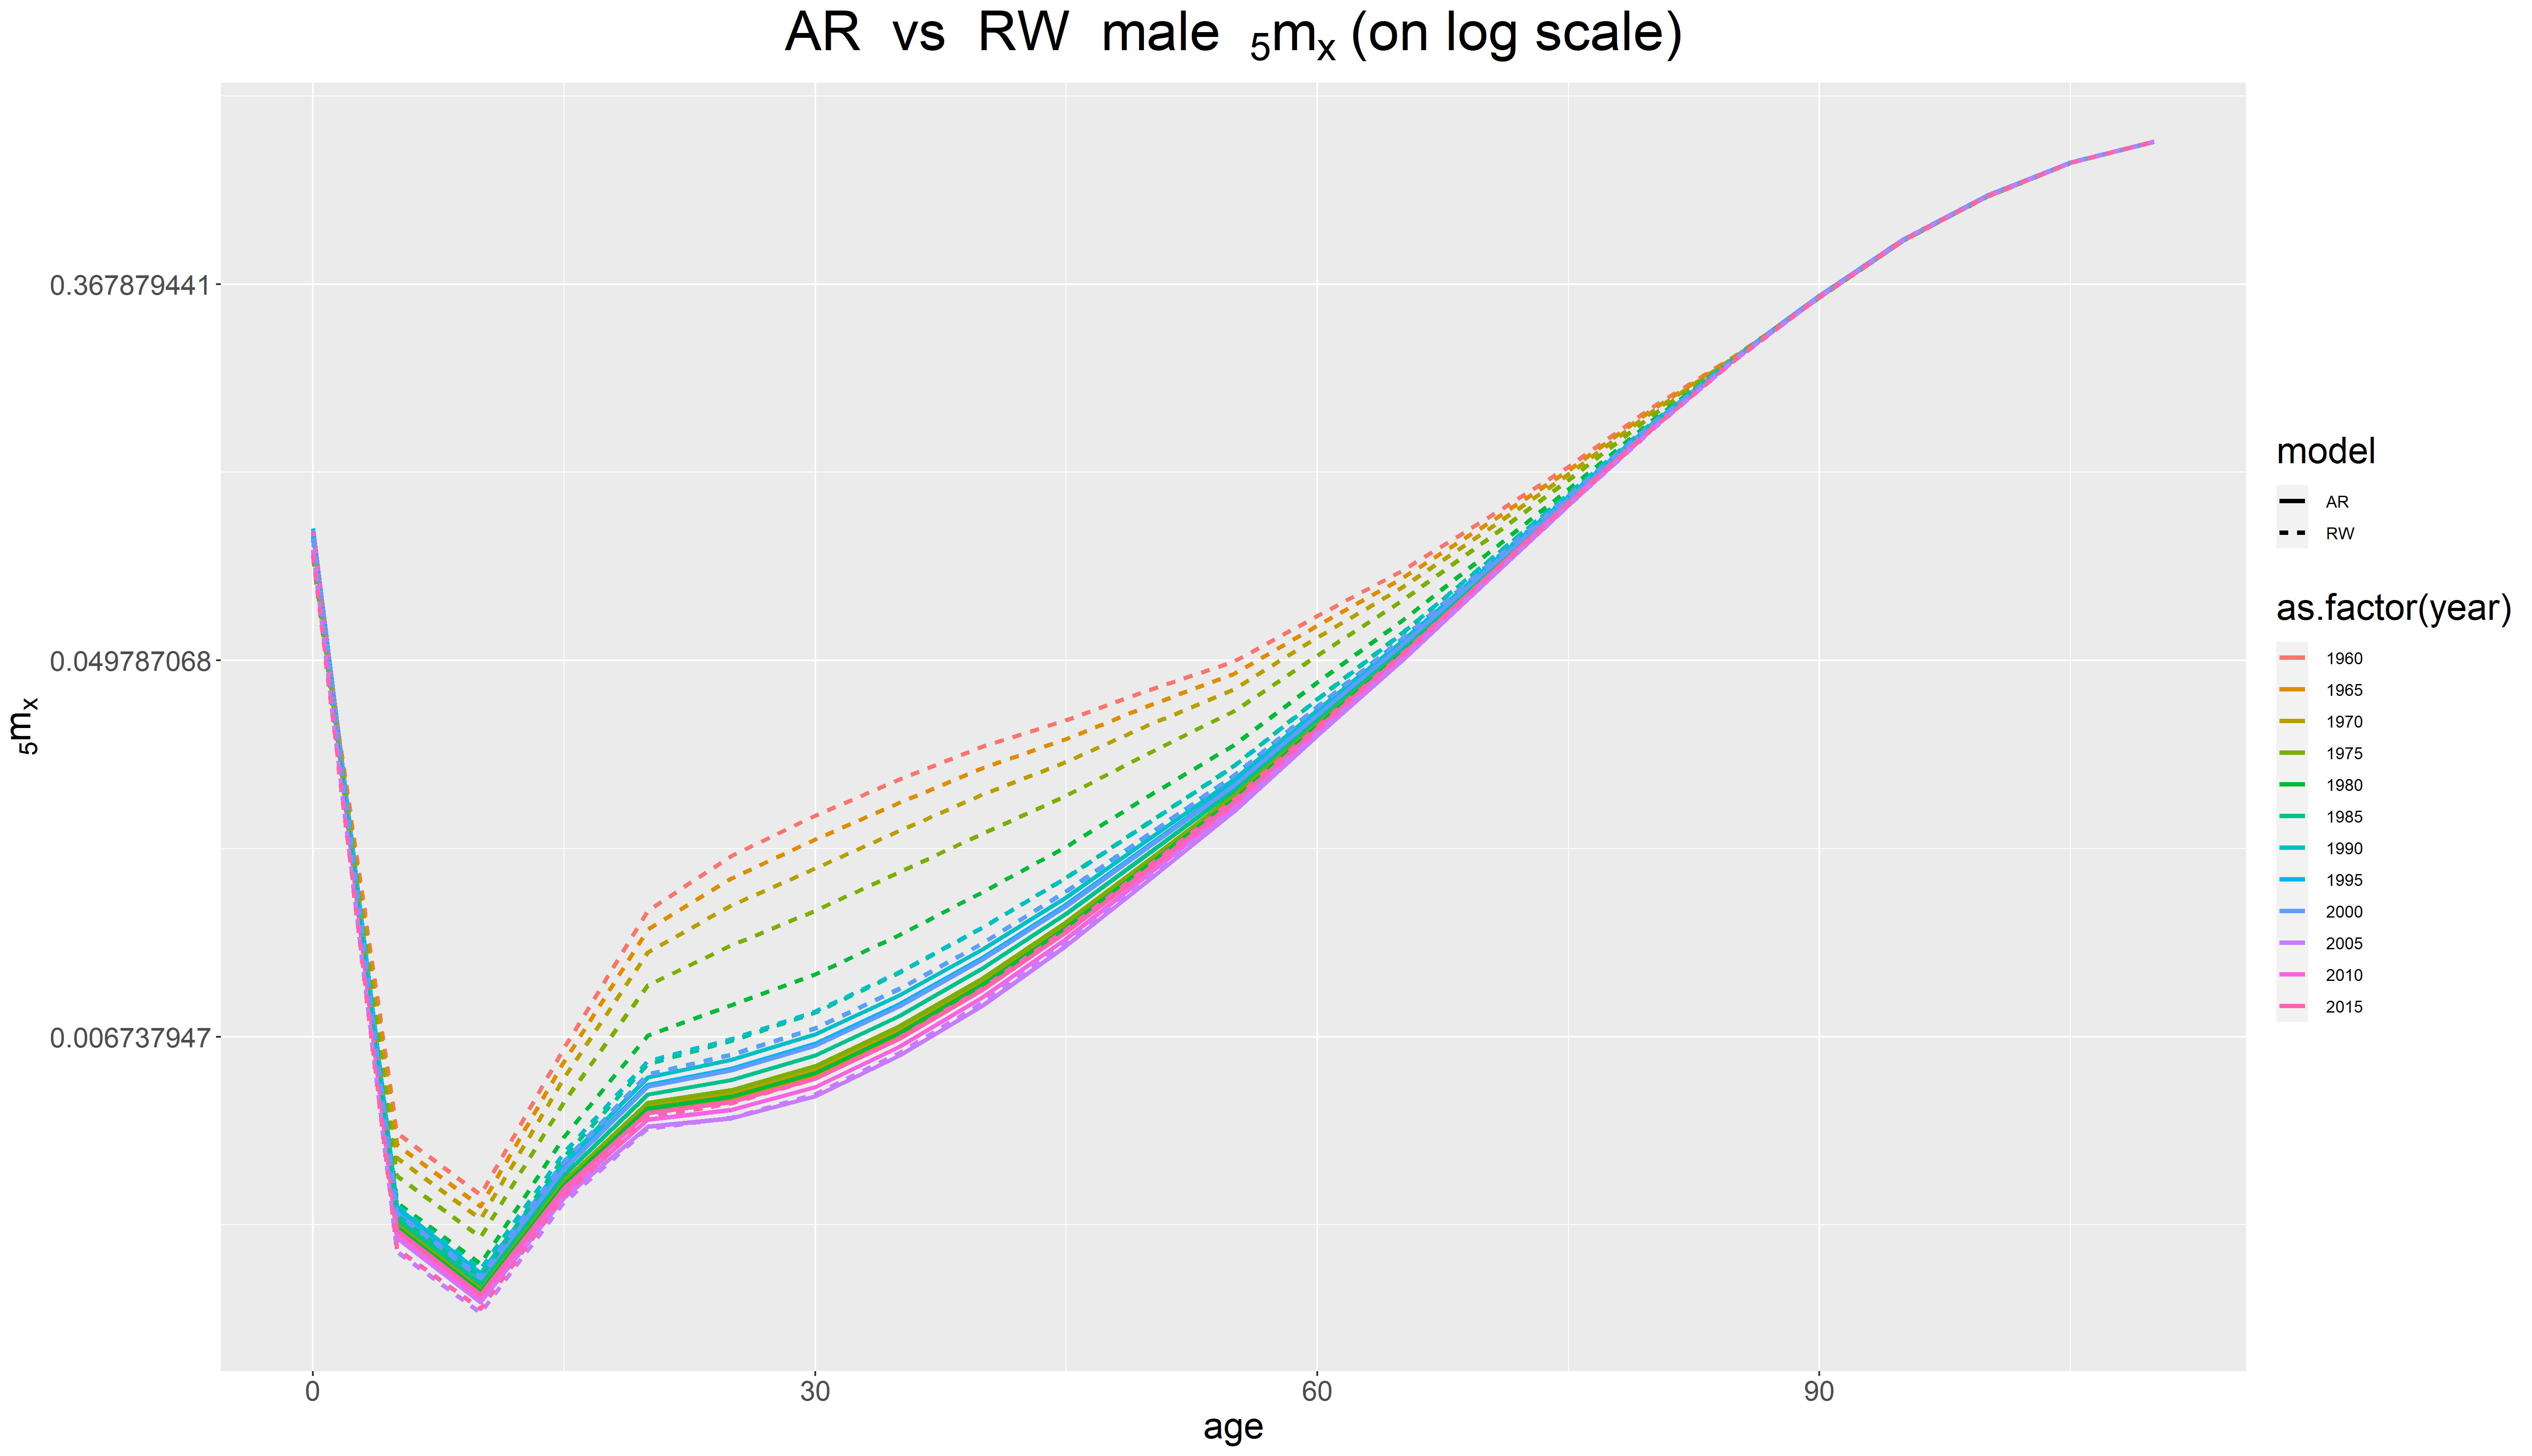
\includegraphics[width=\linewidth]{Burkina Faso/2/compare RW males year.png}
\end{figure}
\begin{figure}[H]
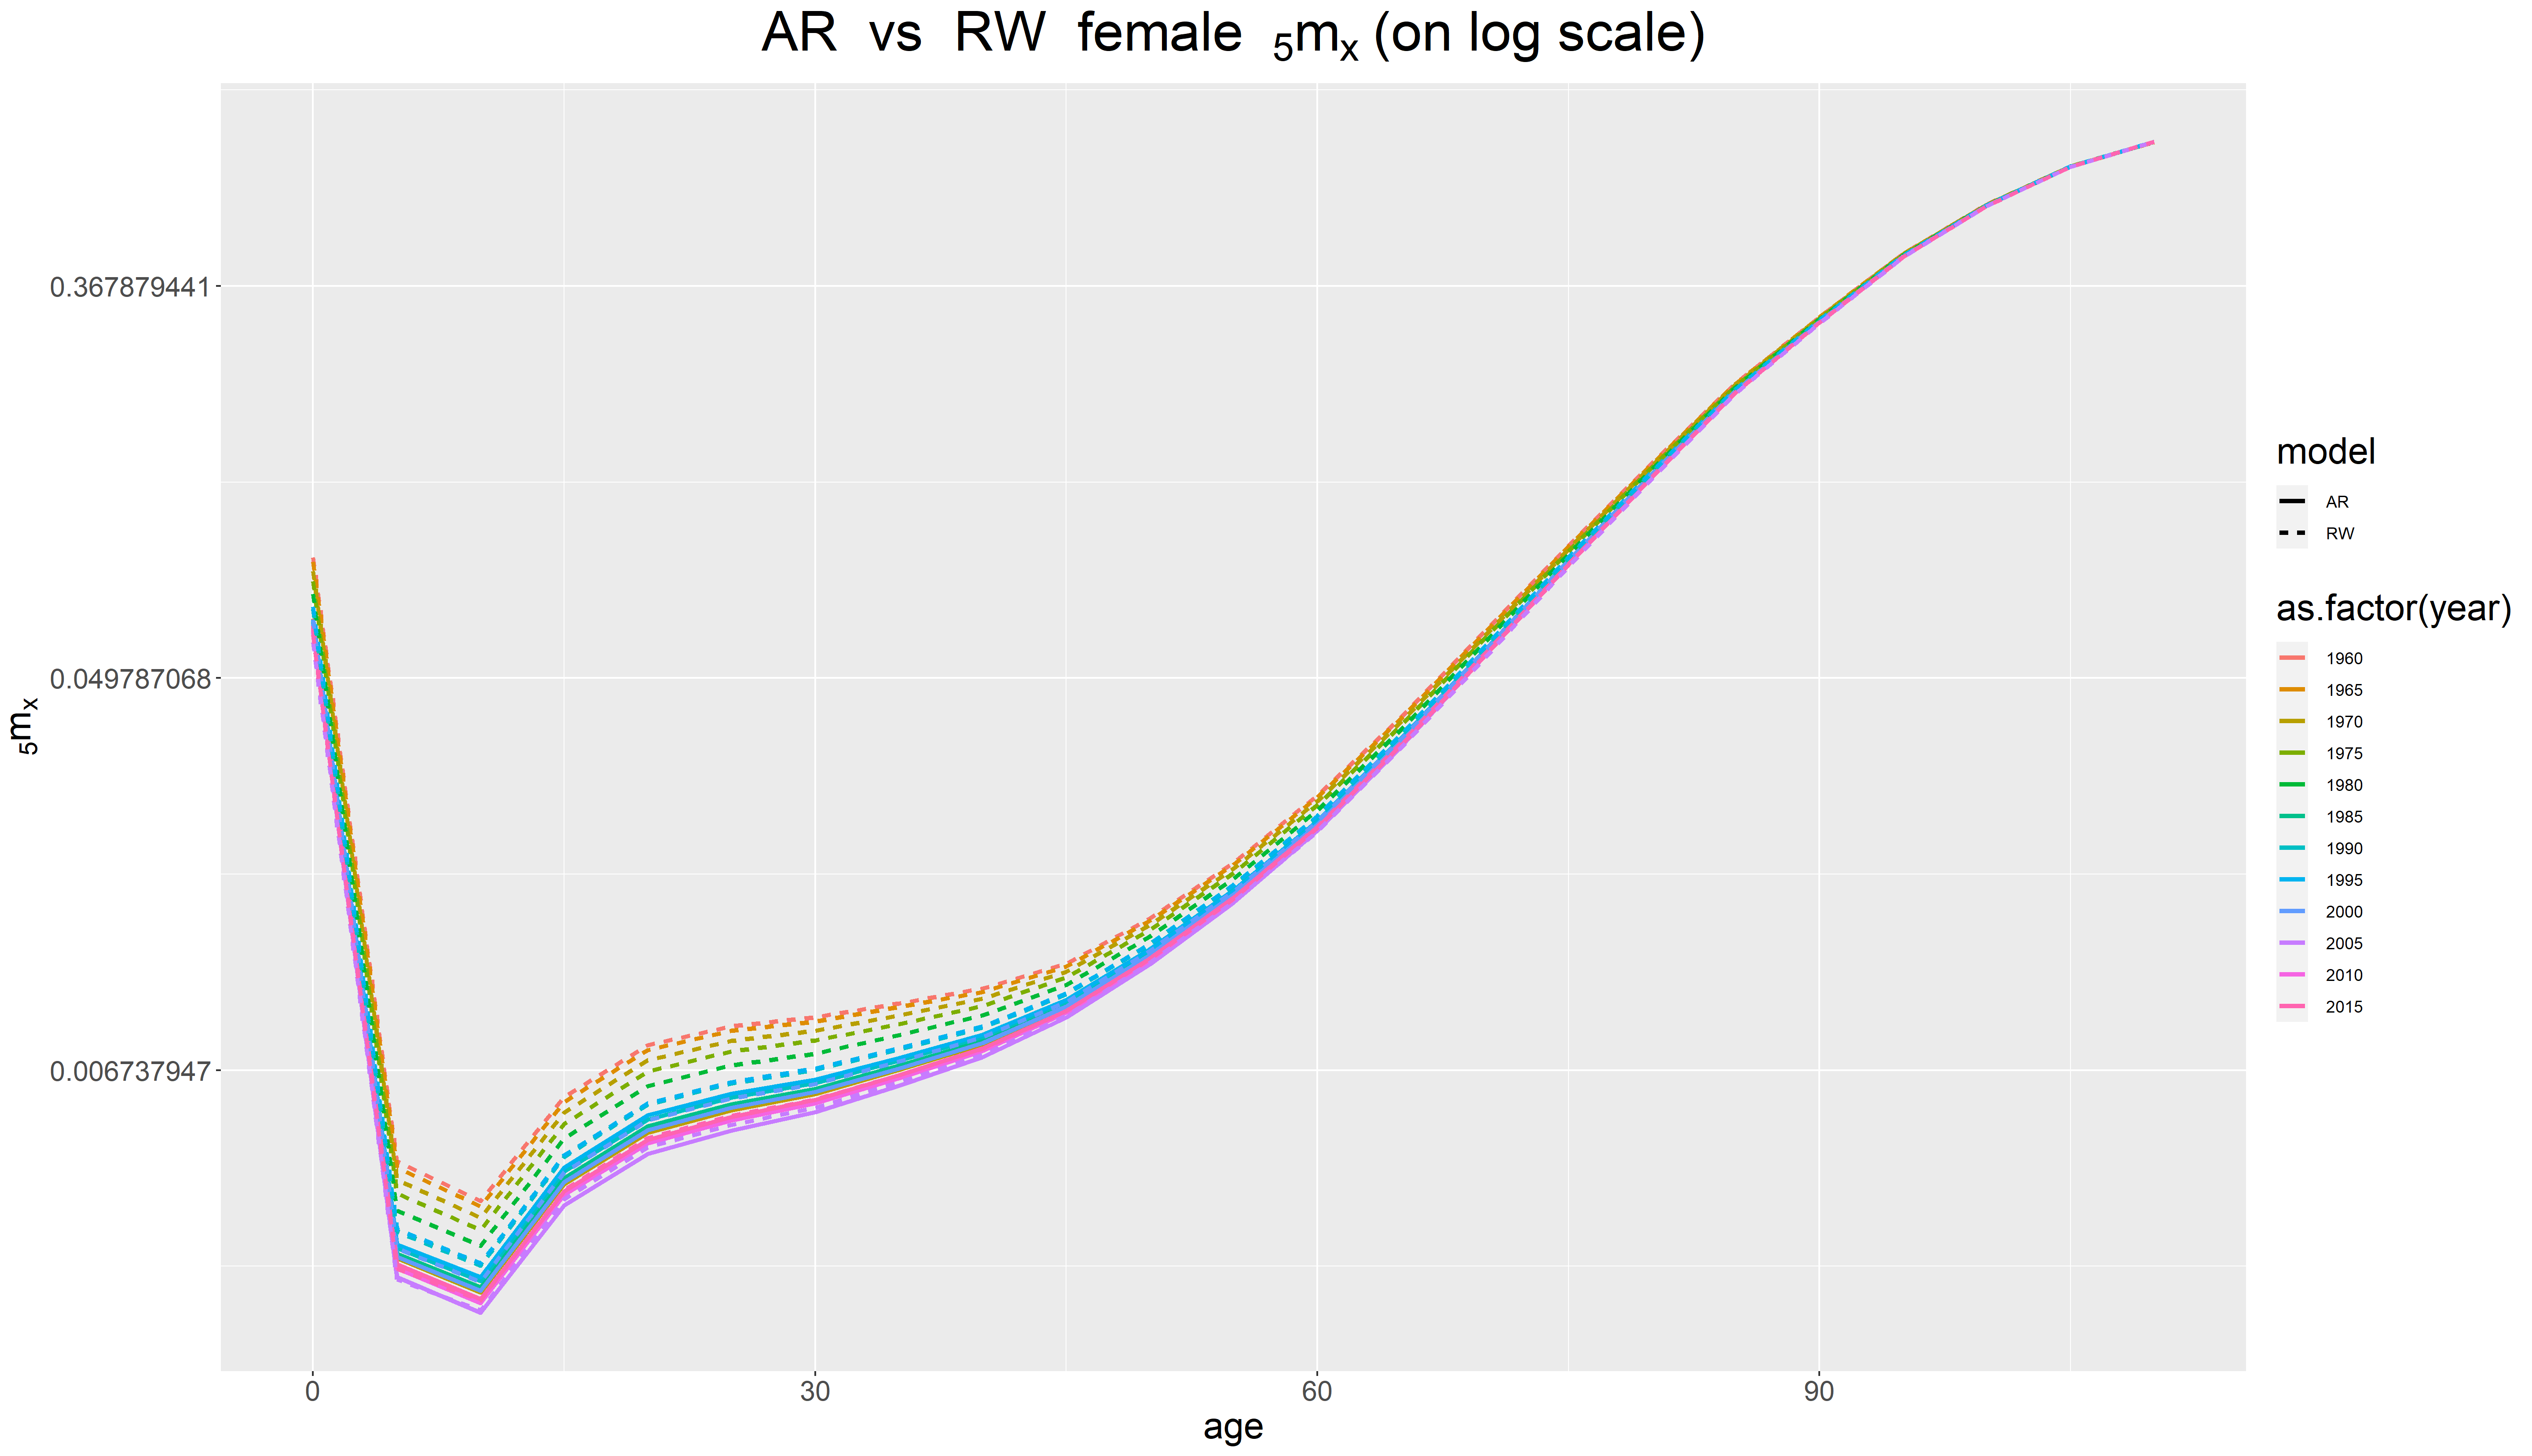
\includegraphics[width=\linewidth]{Burkina Faso/2/compare RW females year.png}
\end{figure}

\end{document} 